\documentclass[jou]{apa6}

\usepackage[american]{babel}

\usepackage{csquotes}
\usepackage[style=apa,sortcites=true,sorting=nyt,backend=biber]{biblatex}
\DeclareLanguageMapping{american}{american-apa}
\addbibresource{bibliography.bib}


%%%%%%%%%%%%%%%%%%%%%%%%%%%%%%%%%%%%%%%%
%% Discrete Structures
%% The start of RBS stuff
%%%%%%%%%%%%%%%%%%%%%%%%%%%%%%%%%%%%%%%%

% Working internal and external links in PDF
\usepackage{hyperref}
% Extra math symbols in LaTeX
\usepackage{amsmath}
\usepackage{gensymb}
\usepackage{amssymb}
% Enumerations with (a), (b), etc.
\usepackage{enumerate}

\let\OLDitemize\itemize
\renewcommand\itemize{\OLDitemize\addtolength{\itemsep}{-6pt}}

\usepackage{etoolbox}
\makeatletter
\preto{\@verbatim}{\topsep=3pt \partopsep=3pt }
\makeatother

% These sizes redefine APA for A4 paper size
\oddsidemargin 0.0in
\evensidemargin 0.0in
\textwidth 6.27in
\headheight 1.0in
\topmargin -24pt
\headheight 12pt
\headsep 12pt
\textheight 9.19in



\setlength\parindent{0pt}

\title{Sample Quiz 4}
\author{Discrete Structures, Fall 2020}
\affiliation{RBS}

\leftheader{Discrete Sample Quiz 4}

\abstract{%
}

%\keywords{}

\begin{document}

\thispagestyle{empty}

\twocolumn
{\Large Preparation for Midterm}

Midterm may contain 3-5 computation problems \textendash{}
Part A, and also 1-2 analysis problems \textendash{} Part B and/or 
1-2 proofs (see Part C). Expect around 8 problems in the midterm (it would be 
about 15 minutes per problem). 

This document is {\bf not} a mock exam; it contains $42$ sample questions
(many more than you would expect to get in actual midterm). This material 
is meant for discussion in order to prepare and to show some variations of the 
problems.

Proofs will closely follow some pattern that has been shown in a homework 
exercise (a variant of an existing proof). 
Also the computation and analysis tasks will follow a 
recognizable pattern that is presented in this preparation material 
or any of the quizzes or homeworks.

%Midterm might contain various types of tasks: 
%Computational Problems (applying algorithms in one
%particular situation); Analysis tasks (for example, 
%express something with predicates or quantifiers or apply some
%other conceptual knowledge); Proofs (showing that 
%some statement is always true). 

%Even, if you are following a known procedure or a proof pattern, 
%you need to add comments to explain what you are doing. 
%They can earn you some points, 
%even if your result turns out incomplete.

% Computation example (15 + 15 + 15 + 15)
% Analysis of a situation (20 + 20) 
% General proof (25 + 25)  

\section{Part A. Computational Problems}

In this part we apply known algorithms to particular situations. 
The goal is to obtain correct result and and add a short explanation, what 
you did and why.

\subsection{A1. Propositional Logic}

{\bf Question 1.} 
Consider this Boolean expression: $E = p \rightarrow q \rightarrow r$. 
Implication ($\rightarrow$) is right-associative. 
\begin{enumerate}[(a)]
\item Write an equivalent Boolean expression using only conjunctions ($\wedge$) and negations ($\neg$). 
\item Fill in the missing parts in the truth table:\\
\begin{tabular}{ c | c | c | c }
$p$ & $q$ & $r$ & $E$ \\ \hline
{\tt T} & {\tt T} & {\tt T} & $\ldots$ \\ \hline
{\tt T} & {\tt T} & {\tt F} & $\ldots$ \\ \hline
{\tt T} & {\tt F} & {\tt T} & $\ldots$ \\ \hline
{\tt T} & {\tt F} & {\tt F} & $\ldots$ \\ \hline
{\tt F} & {\tt T} & {\tt T} & {\tt T} \\ \hline
{\tt F} & {\tt T} & {\tt F} & {\tt T} \\ \hline
{\tt F} & {\tt F} & {\tt T} & {\tt T} \\ \hline
{\tt F} & {\tt F} & {\tt F} & {\tt T} \\ \hline
\end{tabular}
\end{enumerate}

\vspace{6pt}
{\bf Question 2.} 
Assume the following precedence order and associativity of the $5$ Boolean operations: 

\begin{tabular}{lll}
{\tt \textasciitilde{}a} & 1st precedence & right-associative \\
{\tt a/\textbackslash{}b} & 2nd precedence & right-associative \\
{\tt a\textbackslash{}/b} & 3rd precedence & right-associative \\
{\tt a<->b} & 4th precedence & left-associative \\
{\tt a->b} & 5th precedence & right-associative 
\end{tabular}

Show step-by-step how would you restore parentheses in the following 
Boolean expression (each step adds one pair of parentheses \textendash{}
in the order that follows from the rules of precedence 
and associativity):\\
{\tt a -> b /\textbackslash{} \textasciitilde{} c 
\textbackslash{}/ \textasciitilde{} \textasciitilde{} d 
<-> e -> f <-> g}


\vspace{6pt}
{\bf Question 3.} The following syntax tree shows different options how 
$5$ people \textendash{} Bill, John, Jim, Simon and Mike \textendash{} can 
work in a yard. (Variable {\tt Bill} is true iff Bill works in the yard, 
and the whole expression evaluates to true, iff it shows a possible combination
how a team of boys can work in the yard). 
\begin{center}
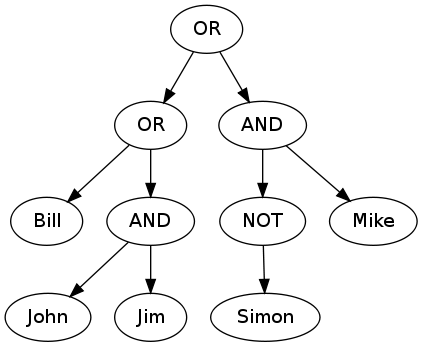
\includegraphics[width=2in]{midterm/syntax-tree.png}
\end{center}
\begin{enumerate}[(A)]
\item Write this tree as a Boolean expression using 
Boolean connectives ($\neg$, $\wedge$, etc.).
\item Write the same expression and ensure that it does not 
use any unnecessary parentheses (precedence and associativity is 
same as in Question 2). 
\item Write an equivalent expression using just two Boolean 
connectives (negation $\neg$ and disjunction $\vee$). 
\end{enumerate}


\subsection{A2. Sets and Quantifiers}

{\bf Question 4.} 
The universe $U$ is all integers between $1$ and $600$. 
$K_2 \subseteq U$ denotes all even numbers from $U$.
Similarly, $K_3 \subseteq U$ denotes all numbers divisible by $3$; 
$K_5 \subseteq U$ denotes all numbers divisible by $5$. 

\begin{enumerate}[(A)]
\item Draw Euler-Venn diagram with a big rectangle (the set $U$), 
the subsets $K_2$, $K_3$, $K_5$ as three intersecting circles.
\item Shade the region that corresponds to the set
$(K_2 \cap \overline K_3) \cup K_5$. 
\item Find the cardinality of the set
$\left| (K_2 \cap \overline K_3) \cup K_5 \right|$, 
justify your answer. 
\item Describe, which elements are in the set 
$(K_2 \cap \overline K_3) \cup K_5$ in English. 
For example: {\em ``All ... such that ... is divisible ... 
and/or is not divisible...''}. 
\end{enumerate}

\vspace{6pt}
{\bf Question 5.} 
In these pictures a red square on the intersection 
of row $i$ and column $j$ 
means that the predicate $L(i,j)$ is true (person $i$ 
loves person $j$). White square means that the predicate $L(i,j)$
is false. Here 
$i,j \in \{ \mathtt{a},\mathtt{b},\mathtt{c},\mathtt{d},\mathtt{e} \}$. 
\begin{center}
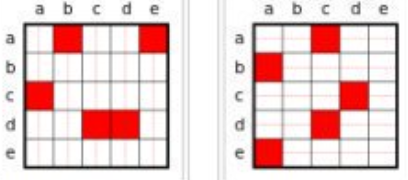
\includegraphics[width=2in]{midterm/predicate-grid.png}
\end{center}
Which statement is shown in the left picture?
\begin{enumerate}[(A)]
\item Everyone is loved by someone.
\item Eveyone loves someone.
\item Someone loves everyone.
\item Someone is loved by everyone.
\end{enumerate}
Which statement is shown in the right picture?
\begin{enumerate}[(A)]
\item $\forall x\, \exists y,\;L(y,x)$. 
\item $\forall x\, \exists y,\;L(x,y)$. 
\item $\exists x\, \forall y,\;L(x,y)$. 
\item $\exists x\, \forall y,\;L(y,x)$. 
\end{enumerate}




\subsection{A3. Algorithms and Big-O Notation}

In these problems you can verify the definition of the Big-O Notation 
or find the limit $f(n)/g(n)$ as $n \rightarrow \infty$. 

{\bf Question 6.} For each function find the smallest
$k$ such that $f(n)$ is in $O(n^k)$. Justify your answer.
\begin{enumerate}[(A)]
\item $f(n) = \sum_{j=1}^{n} (j^3 + j \log_2 j)$. 
\item $f(n) = n^3 + \sin n^7$. 
\item $f(n) = 1^2 + 2^2 + \ldots + n^2$.
\end{enumerate}

\vspace{6pt}
{\bf Question 7.} We say that the functions $f(n)$ and $g(n)$
{\em are of the same order}, if $f(n)$ is in $O(g(n))$ and
$g(n)$ is in $O(f(n))$. Find all pairs of functions in this 
list that are of the same order:
$$n^2 + \log_2 n,\; 2^n + 3^n,\; 100n^3 + n^2,\; n^2 + 2^n,$$
$$n^2 + n^3,\;3n^3 + 2^n.$$






\subsection{A4. Number Theory}


{\bf Question 8.}
\begin{enumerate}[(A)]
\item
Somebody has written a long hexadecimal number
{\tt F0F0F0...F0F} \textendash{} it uses $28$ digits "F"
separated by $27$ digits "0". 
Express the value of this number as a short expression
(without $\ldots$), using
the formula of a geometric progression: $\frac{b_1(q^{n+1}-1)}{q - 1}$. 
\item 
Somebody has written an infinite hexadecimal fraction 
{\tt 0.F0F0F0\ldots}. Express it as a rational number in 
decimal notation. 
\end{enumerate}



\vspace{6pt}
{\bf Question 9.} 
\begin{center}
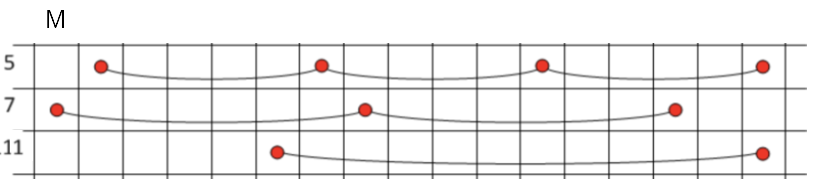
\includegraphics[width=3in]{midterm/sequences.png}
\end{center}

\begin{enumerate}[(A)]
\item Find some number $M \in \mathbb{Z}^{+}$ 
that gives the following remainders when divided by 
$5$, $7$ and $11$: 
$$\left\{
\begin{array}{l}
M \equiv 4\;(\text{mod}\,5)\\
M \equiv 0\;(\text{mod}\,7)\\
M \equiv 6\;(\text{mod}\,11)
\end{array} \right.$$
\item Find the arithmetic progression containing all such numbers $M$.
\end{enumerate}



\vspace{6pt}
{\bf Question 10.} 
\begin{enumerate}[(A)]
\item Alice has $13$-cent coins; Bob has $21$-cent coins. 
Alice wants to pay Bob exactly $1$ cent. How to do this?
\item Alice has $21$-cent coins; Bob has $13$-cent coins. 
Alice wants to pay Bob exactly $1$ cent. How to do this?
\item Solve the congruence equation \textendash{} find
$x$ such that $13x \equiv 1\;(mod\;21)$. 
\item Solve the congruence equation \textendash{} find
$x$ such that $13x \equiv 4\;(mod\;21)$. 
\end{enumerate}


\vspace{6pt}
{\bf Question 11.} 
\begin{enumerate}[(A)]
\item Write all positive powers of number $2$ ($2^1, 2^2, 2^3,\ldots$) modulo $11$ until 
you find a loop: i.e. some remainder repeats itself. How long is the period?
\item Write all negative powers of number $2$ modulo $13$ ($2^{-1},2^{-2},2^{-3},\ldots$) until 
you find a loop. How long is the period?
\end{enumerate}

{\em Note.} A negative power, for example $2^{-k}$ is such that $2^{-k}\cdot 2^k \equiv 1\;(\text{mod}\;11)$. 





\section{Part B. Analysis Tasks}

In these problems you have to apply concepts 
(such as predicates or quantifiers) to new situations, 
describe algorithms or procedures for new tasks
or sort cases in adaptive ways.


\subsection{B1. Propositional Logic}

{\bf Question 12.}
Among the people $A,B,C$ one is a truth-teller, 
the other two are liars. 
Every person ($A$, $B$, and $C$) has a closed box
in front of himself/herself. Exactly one of the 
boxes has a candy inside. $A,B,C$ know everything 
about each other and the location of candy.\\
Find out, which YES/NO questions you 
need to ask to find out, which box contains candy. 
Ask as few questions as possible 
(``brute-force'' strategies that ask clearly redundant
questions may only get partial credit). 

\vspace{6pt}
{\bf Question 13.} 
\begin{enumerate}[(a)]
\item Find out, if this formula is a tautology: 
$$\mathtt{((A \vee B) \wedge (A \rightarrow C) \wedge 
(B \rightarrow C)) \rightarrow C}.$$
\item Find out, if this formula is satisfiable: 
$$\mathtt{\neg (((A \vee B) \wedge (A \rightarrow C) \wedge 
(B \rightarrow C)) \rightarrow C)}.$$
\end{enumerate}

{\em Note.} A Boolean expression is called {\em tautology}, 
if it is true for all 
possible truth values of its variables. 
An expression is called {\em satisfiable}, 
if there is a way to assign 
variables so that it becomes true. 

\vspace{6pt}
{\bf Question 14.} 
Let us have three people \textendash{} Ada, Barbara and Cecilia. 
Every day some of them are charging batteries for Lego robots.
Let us have propositional variables $a,b,c$ (a variable $a,b,c$ is true, iff 
today batteries were charged by Ada, Barbara or Cecilia respectively). 

Write a Boolean expression telling that today batteries were charged
by {\bf exactly} two people out of the three. You can use variables $a,b,c$ and
all $5$ Boolean connectives ($\neg$, $\vee$, $\wedge$, $\rightarrow$, 
$\leftrightarrow$). 



\subsection{B2. Sets and Quantifiers}

{\bf Question 15.} We define the set of all bounded functions defined on the interval $(a;b)$ 
as functions that have all their values between two bounds: there is a positive number $M$
such that all all values of the function $f$ are in the interval $[-M;M]$. With predicates and quantifiers:
$$\exists M \in \mathbb{R}^{+},\,\forall x \in \mathbb{R}\,\;x \in (a;b) \rightarrow |f(x)| \leq M.$$
In this picture one of the functions (the red one) is bounded, the other one is unbounded.
\begin{center}
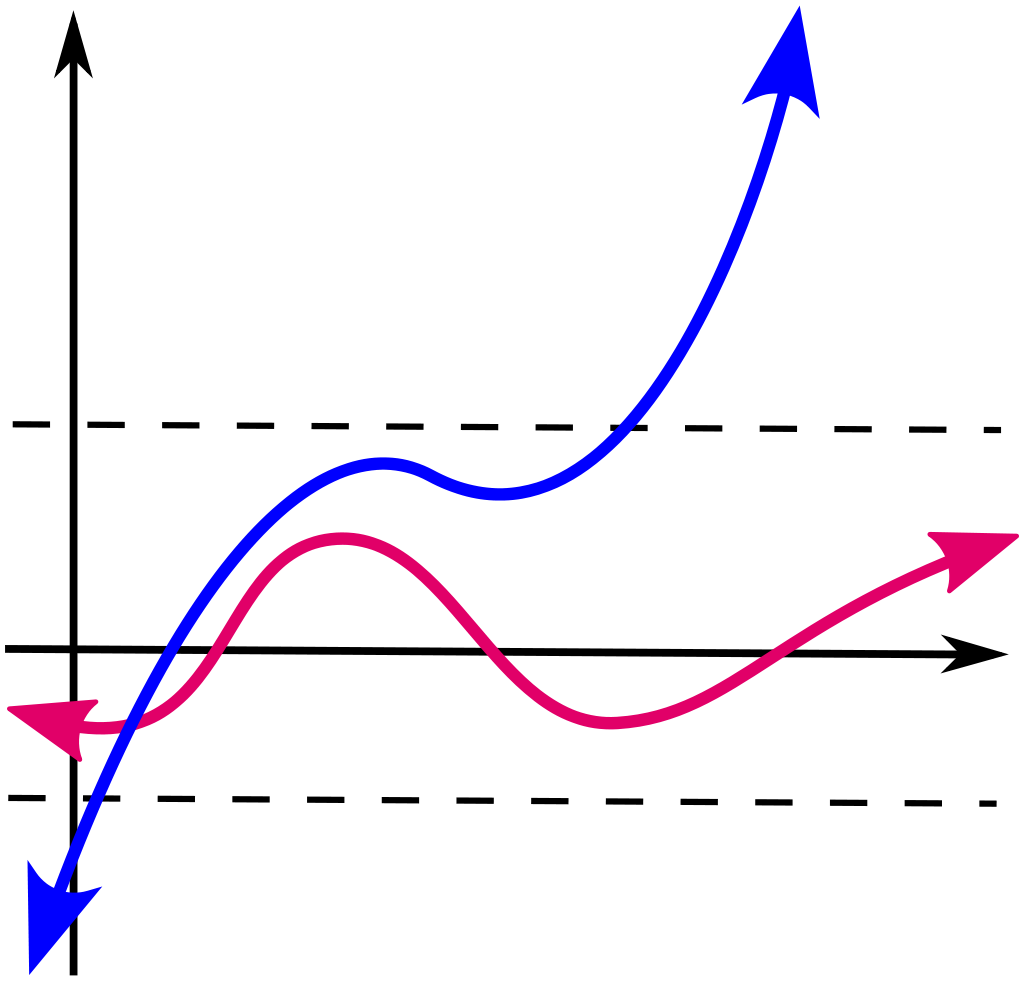
\includegraphics[width=2in]{midterm/bounded-function.png}
\end{center}
\begin{enumerate}[(A)]
\item Write an expression with predicates and quantifiers to express the statement: 
``Function $f:(a;b) \rightarrow \mathbb{R}$ is {\bf not} bounded.''
\item Find an example of a function that is defined and bounded in the interval $(0;1)$. 
\item Find an example of a function that is defined, but unbounded in the interval $(0;1)$. 
\item What functions are described by another predicate logic expression, where we switch the order of quantifiers:
$$\forall x \in \mathbb{R}\,\exists M \in \mathbb{R}^{+},\;x \in (a;b) \rightarrow |f(x)| \leq M.$$
\end{enumerate}


\vspace{6pt}
{\bf Question 16.} An infinite sequence $a_0,a_1,a_2,\ldots$ is called {\em purely periodic}, if 
all the members of it repeat the same finite pattern over and over again. 
For example, $3,3,3,3,\ldots$ or $1,3,1,3,1,3,\ldots$ are purely periodic. 
Meanwhile, 
$1,6,6,6,6,\ldots$ or $1,4,1,4,2,1,3,5,\ldots$ (the digits of $\sqrt{2}$) 
are not purely periodic (they are either ``eventually periodic'' with some digits preceding the period 
or not periodic at all). 
\begin{enumerate}[(A)]
\item Write an expression to tell that a given sequence $(a_n)_{n \in \mathbb{N}}$ 
is purely periodic. 
\item Write an expression to tell that a given sequence $(a_n)_{n \in \mathbb{N}}$ 
is {\bf NOT} purely periodic. 
\end{enumerate}


\vspace{6pt}
{\bf Question 17.} 
Consider the set $A = \{ 1,2,3,4,6,12 \}$. We define a
predicate 
$$P \,:\, A \times A \rightarrow \{ \mathtt{True}, \mathtt{False} \},$$
where $P(i,j)$ is true iff the divisibility by $i$ implies 
divisibility by $j$ (for any $i,j \in A$). 
For example $P(12,2) = \mathtt{True}$, since any number 
that is divisible by $i = 12$ is also divisible by $j=2$. 

\begin{enumerate}[(A)]
\item Is the 2-argument predicate $P$ {\em reflexive} \textendash{}
does it satisfy the logic formula:
$$\forall i \in A,\;P(i,i).$$
\item Is the predicate $P$ {\em symmetric} \textendash{}
does it satisfy the logic formula:
$$\forall i \in A,\,\forall j \in A,\;P(i,j) \rightarrow P(j,i).$$
\item Is the predicate $P$ {\em transitive} \textendash{}
does it satisfy the logic formula:
$$\forall i,j,k \in A,\;P(i,j) \wedge P(j,k) \rightarrow P(i,k).$$
\item Is the predicate $P$ {\em connex} \textendash{}
does it satisfy the logic formula:
$$\forall i,j \in A,\;P(i,j) \vee P(j,i).$$
\end{enumerate}

{\em Note 1.} Even though the predicate formulas can be verified
by checking all possible combinations of $i,j,k \in A$ (the set $A$ is finite), 
it is much faster to reason by the properties of divisibility.\\
{\em Note 2.} For each statement either add a short justification or provide
a counterexample.






\subsection{B3. Algorithms and Big-O Notation} 

{\bf Question 18.} Let $A,B$ be subsets from the same universe $U = \{ 1,2,\ldots,n \}$. 
We want to find the intersection of these two sets $A \cap B$. 

\begin{enumerate}[(A)]
\item Describe an algorithm (using steps written in English or some pseudocode) 
to find and to output all numbers that are in this intersection $A \cap B$. 
(You can call the algorithms that are in the K.Rosen's textbook - for sorting, 
linear or binary search and similar. But write out your assumptions, so that it is unambiguous, 
which method you are using.)
\item Estimate the time complexity $O(f(n))$: provide a function that estimates the 
worst-case time required as the size of the universe $U$ grows.
\end{enumerate}

\vspace{6pt}
{\bf Question 19.} 
\begin{enumerate}
\item 
Prove that $f(n) = n^2 + n \cdot \ln n$ is in $O(n^2)$ (i.e. $g(n) = n^2$) by finding the limit
of the ratio:
$$\lim_{n \rightarrow \infty} \frac{n^2 + n \cdot \ln n}{n^2}.$$
Or by directly checking the definition of the Big-O notation (finding the two 
constants $C$ and $k$ that give you the estimate: 
$n>k \rightarrow |f(n)| \leq C|g(n)|$.
\item Is the function $g(n) = n^2$ also in $O(f(n))$, where $f(n) = n^2 + n \cdot \ln n$? 
Once again, justify by finding a limit or by checking the definition.
\end{enumerate}





\subsection{B4. Number Theory} 


{\bf Question 20.} Let us consider the following statement:\\

{\bf Bezout's identity:} 
Let $a$ and $b$ be integers and $d$ is their greatest common divisor: $\text{gcd}(a,b)=d$. 
Then, there exist integers $x$ and $y$ such that $ax + by = d$.\\

\begin{enumerate}[(A)] 
\item Let us have parameters $a,b \in \mathbb{Z}$ and $d \in \mathbb{Z}^{+}$ such that $\text{gcd}(a,b)=d$. 
Write the Bezout's identity using predicates and quantifiers (you can also 
use equality and four arithmetic operations). 
\item Using the same notation as before, write another statement using predicates and quantifiers: 
``The modular equation $ax\equiv{}c\;(\text{mod}\,b)$ has a solution if and only if 
$c$ is a multiple of $d$.''
\item Using the same notation as before, write another statement using predicates and quantifiers: 
``The greatest common divisor $d$ is the smallest positive integer that can be expressed as $ax+by$ for 
the given $a,b$ and any integers $x,y$.''
\end{enumerate}

{\em Note 1.} In this expression $a,b,c,d$ are {\em free variables}; they are given and can be used in your formulas. 
You can also use any number of {\em bound variables}.\\
{\em Note 2.} We call $c$ a {\em multiple} of $d$ iff $c$ can be expressed as some integer number times $d$.

\vspace{6pt}
{\bf Question 21.} Somebody has proposed a way to encode finite sequences of natural numbers $\mathbb{N}$
(i.e. nonnegative integers: $\mathbb{N} = 0,1,2,\ldots$) as natural numbers. 
To encode a sequence $(a_1,a_2,\ldots,a_k)$ we take the first $k$ primes
($p_1 = 2$, $p_2 = 3$, $p_3 = 5$, and so on) and build a number: 
$$f(a_1,a_2,\ldots,a_k) = p_1^{a_1}p_2^{a_2}p_3^{a_3}\ldots$$
For example, the sequence $(1,0,2)$ is encoded as $2^1\cdot{} 3^0 \cdot 5^2 = 50$, 
but the sequence $(1,1,1,1)$ is encoded as $2^1 \cdot 3^1 \cdot 5^1 \cdot 7^1 =  210$.
\begin{enumerate}
\item Is the function $f: \mathbb{N}^{\ast} \rightarrow \mathbb{N}$ a surjection?
\item Is the function $f: \mathbb{N}^{\ast} \rightarrow \mathbb{N}$ an injection?
\item Can you suggest a bijective function $g: \mathbb{N}^{\ast} \rightarrow \mathbb{N}$ to encode any finite sequence of natural numbers 
with a single natural number?
\end{enumerate}

{\em Note.} By $\mathbb{N}^{\ast}$ we denote a list of all finite tuples: 
$$\mathbb{N}^{\ast} = \{()\} \cup (\mathbb{N}) \cup (\mathbb{N} \times \mathbb{N}) \cup \ldots.$$
It contains one list of length $0$,\\
It contains $(\mathbb{N})$ all single-element lists $(0)$, $(1)$, etc.,\\
It contains $(\mathbb{N} \times \mathbb{N})$, i.e. all two-element pairs $(0,0)$, $(0,1)$, $(1,0)$, $(1,1)$, etc.\\
And so on.

\vspace{6pt}
{\bf Question 22.} Consider the set of all square functions ($f:\mathbb{R} \rightarrow \mathbb{R}$)
that can be expressed as $f(x) = ax^2 + bx + c$ with integer coefficients $a,b,c$. 
Is the set of all such square functions finite? countable? uncountable? 
Justify your answer.





\section{Part C. Proofs}

In proof problems the goal is to prove some general statement by 
showing every essential step of your reasoning.
Below we describe various proof strategies and give some sample
statements that can be proven by that strategy.

\vspace{6pt}
{\bf Translate into Algebra}

In K.Rosen's textbook these are called ``direct proofs''
of IF-THEN statements. 
You assume that the condition is true, introduce some notation and 
prove that also the conclusion is true.
You sometimes need to sort cases. 

\vspace{6pt}
{\bf Question 23.} Prove that, if $n$ is odd, then $n^2$ is also odd. 

\vspace{6pt}
{\bf Question 24.} Prove that, if the decimal notation of a number $n$ ends with the digit "5", 
then $n^2$ ends with digits "25". 

\vspace{6pt}
{\bf Question 25.}
Prove that $n^2 \equiv 5\;(\text{mod}\;11)$ is true
iff
$n \equiv 4\;(\text{mod}\;11)$ 
or $n \equiv -4\;(\text{mod}\;11)$.

\vspace{20pt}
{\bf Proofs by Contradiction}

In these examples you assume that the statement is false
and get a contradiction.


\vspace{6pt}
{\bf Question 26.} Prove that there are infinitely many primes.

\vspace{6pt}
{\bf Question 27.} Prove that there are infinitely many primes of the form $4n+3$. 

\vspace{6pt}
{\bf Question 28.} Prove that there are infinitely many primes
that divide some value of the polynomial 
$P(n) = n^2 + n + 1$. 

\vspace{6pt}
{\bf Question 29.}
Prove that $\sqrt{2}$ is irrational.

\vspace{6pt}
{\bf Question 30.}
$\log_2 10$ is irrational.


\vspace{20pt}
{\bf Building Bijective Functions (Countable)}

Any combinations of these tactics can be used
to prove that two sets have the same cardinality
(and that there is a bijective function from one set to another).

\vspace{6pt}
{\bf Question 31.}
There is a bijection from $\mathbb{Z}^{+} \cup \{ 1,2,\ldots,n \}$
to $\mathbb{Z}^{+}$.\\
{\em Hint.} One can add $n$ new guests to the Hilbert's hotel.

\vspace{6pt}
{\bf Question 32.}
There is a bijection from $\mathbb{Z}^{+} \times \{ 1,2 \}$
to $\mathbb{Z}^{+}$.\\
{\em Hint.} If there are two infinite buses with guests: 
$(1,1),(2,1),(3,1),\ldots$ and $(1,2),(2,2),(2,3),\ldots$, 
then they can be hosted in a single Hilbert's hotel.

\vspace{6pt}
{\bf Question 33.}
There is a bijection from $\mathbb{Z}^{+} \times \mathbb{Z}^{+}$
to $\mathbb{Z}^{+}$.\\
{\em Hint.} Show how infinitely many infinite buses can be hosted in a 
single Hilbert's hotel (similar to Question 9 from HW1).

\vspace{6pt}
{\bf Question 34.}
There is a bijection from $\mathbb{Q}$ to $\mathbb{Z}^{+}$.\\
{\em Hint.} Same as above, but now you need to combine
three sets of numbers into the same Hilberts hotel (positive rationals, 
negative rationals and $0$). 

\vspace{20pt}
{\bf Building Bijective Functions (Uncountable)}

\vspace{6pt}
{\bf Question 35.}
There is a bijective function from any closed 
segment $[a;b]$ to any other closed segment $[c;d]$
(regardless of their lengths).\\
{\em Hint.} This can be achieved by a simple linear function.

\vspace{6pt}
{\bf Question 36.}
There is a bijective function from any open 
segment $(a;b)$ to any other open segment $(c;d)$.\\
{\em Hint.} This also can be achieved by a linear function. 

\vspace{6pt}
{\bf Question 37.}
There is a bijective function from any open 
segment $(a;b)$ to the set of all real numbers $\mathbb{R}$
or to the half-line of all positive reals $(0;+\infty)$.\\
{\em Hint.} You can use a continuous function with one or two 
vertical asymptotes. Such as $f(x) = x/(1-x)$ or $f(x) = \tan x$.

\vspace{6pt}
{\bf Question 38.}
There is a bijective function from a 
semi-open segment $[0;1)$ to an open segment $(0;1)$.\\
{\em Hint.} Map the extra point (argument $x = 0$) to any 
point inside the target interval $(0;1)$, then 
change values for an infinite sequence (bounded inside $(0;1)$)
in the same way as Hibert's hotel. 


\vspace{20pt}
{\bf Proving there is no Bijection}

All these proofs use Cantor's diagonalization. (See subsection 
``2.5.3 An uncountable set'' in the textbook; pp. 183-187.)

\vspace{6pt}
{\bf Question 39.} Numbers on $(0;1)$ are uncountable.


\vspace{6pt}
{\bf Question 40.}
 All real numbers $\mathbb{R}$ are uncountable - there 
is no bijection from $\mathbb{R}$ to $\mathbb{Z}^{+}$ or
to $\mathbb{Q}$. 


\vspace{6pt}
{\bf Question 41.} All infinite sequences of integers are uncountable
(Also, all non-decreasing sequences of integers are uncountable.


\vspace{6pt}
{\bf Question 42.} The Power-set of any countable set is 
uncountable. For example, 
there is no bijection from $\mathcal{P}(\mathbb{Z}^{+})$
to $\mathbb{Z}^{+}$ (i.e. no mapping from the set of all subsets of 
positive integers to the set of integers themselves).





\end{document}

